% =============================================================================
% NIOT Preliminary Design Report (PDR) — official section order
% 5--10 pages target | Upload zip to Overleaf | main.tex | pdfLaTeX | Download PDF
% Fill [PLACEHOLDERS] on the title page before submission.
% =============================================================================
\documentclass[11pt,a4paper]{article}

\usepackage[margin=2.0cm]{geometry}
\usepackage{amsmath,amssymb}
\usepackage{booktabs}
\usepackage{graphicx}
\usepackage{hyperref}
\usepackage{xcolor}
\usepackage{enumitem}
\usepackage{caption}
\usepackage{fancyhdr}
\usepackage{listings}
\usepackage{float}
\usepackage{setspace}
\usepackage[numbers,sort&compress]{natbib}

\hypersetup{colorlinks=true,linkcolor=black,citecolor=black,urlcolor=blue!50!black}
\pagestyle{fancy}
\fancyhf{}
\fancyhead[L]{\footnotesize Preliminary Design Report}
\fancyhead[R]{\footnotesize NIOT Student Competition}
\fancyfoot[C]{\thepage}
\renewcommand{\headrulewidth}{0.3pt}
\setstretch{1.05}
\lstset{basicstyle=\ttfamily\scriptsize,breaklines=true,frame=single,framesep=2pt}

\begin{document}

%-----------------------------------------------------------------------------
% 1. TITLE PAGE
%-----------------------------------------------------------------------------
\begin{titlepage}
\centering
\vspace*{1.2cm}

{\LARGE\bfseries Preliminary Design Report (PDR)}\\[0.8cm]
{\large National Institute of Ocean Technology (NIOT)\\
Student Autonomous Vehicle Competition}\\[1.2cm]

{\LARGE\bfseries Project Title}\\[0.35cm]
{\Large Cooperative Multi-ASV Magnetic Anomaly Search\\
and Localization using ROS~2 and Gazebo}\\[1.2cm]

\begin{tabular}{@{}ll@{}}
\textbf{Team Registration ID:} & \texttt{[TEAM\_REGISTRATION\_ID]} \\[0.35cm]
\textbf{Institute Name:} & \texttt{[INSTITUTE\_NAME]} \\[0.35cm]
\textbf{Student Name(s):} & \texttt{[STUDENT\_NAME\_1]} \\
 & \texttt{[STUDENT\_NAME\_2]} \\
 & \texttt{[STUDENT\_NAME\_3]} \\[0.35cm]
\textbf{Faculty Mentor Name:} & \texttt{[FACULTY\_MENTOR\_NAME]} \\
\end{tabular}

\vfill
{\large \today}\\[0.5cm]
{\small Submitted through the educational institution as per NIOT guidelines.}
\end{titlepage}

%-----------------------------------------------------------------------------
% 2. ABSTRACT
%-----------------------------------------------------------------------------
\section*{Abstract}
\addcontentsline{toc}{section}{Abstract}
This Preliminary Design Report proposes a \textbf{cooperative multi-Autonomous
Surface Vehicle (ASV)} system for detecting and localizing a compact magnetic
anomaly in a bounded water body. The objectives are: (i)~partitioned survey
coverage with three differential-thrust boats, (ii)~online Bayesian fusion of
cleaned magnetometer anomalies, (iii)~information-driven hunt and densifying
spiral, and (iv)~peer verification before mission completion. The methodology
combines Gazebo Harmonic 3D simulation, ROS~2 Jazzy autonomy nodes, strip
lawnmower path planning, soft-dipole likelihood Bayesian updates, mutual
information waypoint selection, line-of-sight guidance, and a declare/request
verify handshake. Expected outcomes include a completed simulated Phase-4
mission with peer confirmation ($4/4$) and metre-class dipole-fit error against
a planted evaluation target $(85,40)\,\mathrm{m}$, establishing a clear path
from PDR to Phase~I development under NIOT.

%-----------------------------------------------------------------------------
% 3. INTRODUCTION
%-----------------------------------------------------------------------------
\section{Introduction}
\subsection{Background}
Ocean and inland magnetic surveys are used for underwater anomaly detection,
harbour security, and environmental characterization. Autonomous platforms
enable persistent coverage without continuous manned presence. Simulation-led
design reduces risk before hardware Phase~I. This entry uses ROS~2 and Gazebo
Harmonic as the digital twin for a three-ASV magnetic search stack
(\texttt{version\_3} workspace).

\subsection{Problem statement}
Locate an unknown compact magnetic dipole-like anomaly inside a bounded lake
using autonomous craft that \textbf{do not} receive the true target coordinates.
Vehicles must survey cooperatively, fuse weak anomalies ($\sim$ tens of nT) atop
Earth's field ($\sim45{,}000\,\mathrm{nT}$) and sensor noise, then confirm a
candidate before declaring success.

\subsection{Objectives and scope}
\begin{itemize}[leftmargin=*,itemsep=1pt]
  \item Design a multi-ASV cooperative search concept with shared belief and
        peer verification.
  \item Provide theoretical models (dipole, Bayes, information gain, guidance).
  \item Demonstrate the concept in 3D Gazebo simulation with an operator console.
  \item Report preliminary simulation results and Localization error metrics.
  \item Scope of this PDR: simulation-validated architecture for Phase~0/PDR;
        hardware magnetometer integration is Phase~I.
\end{itemize}

%-----------------------------------------------------------------------------
% 4. LITERATURE REVIEW
%-----------------------------------------------------------------------------
\section{Literature Review}
Magnetic anomaly detection with mobile platforms commonly uses dipole forward
models and nonlinear least-squares inversion for localization
\cite{lm}. Autonomous surface craft typically execute boustrophedon (lawnmower)
coverage for hydrography. Informative path planning based on expected entropy
reduction follows Shannon information theory \cite{shannon} and has been applied
to environmental robots. Line-of-sight (LOS) path following is standard for
underactuated marine vehicles. Multi-robot search literature motivates separating
discovery from confirmation to reduce false alarms.

ROS~2 and Gazebo provide reproducible middleware and physics for marine
robotics prototyping \cite{ros2,gz}. Existing works rarely package, in one
competition-ready simulation, (a)~multi-vehicle strip deconfliction,
(b)~online Bayesian magnetic fusion, (c)~mutual-information hunt,
(d)~shore-safe densification, and (e)~peer verify handshakes.

\paragraph{Research gap and motivation.}
There is a need for an integrated, institutionally reproducible ASV magnetic
search pipeline with clear mathematical substantiation and simulation evidence
suitable for NIOT PDR evaluation. This work addresses that gap as a simulation
concept design preparatory to Phase~I development.

%-----------------------------------------------------------------------------
% 5. THEORETICAL DESIGN
%-----------------------------------------------------------------------------
\section{Theoretical Design}
\subsection{Overall system architecture}
\begin{lstlisting}
Gazebo plant (3 ASVs, lake, shores)
   | ros_gz_bridge (odom,imu,gps,mag <-> thrust)
   v
Per-boat /asvN: sensing -> mission_manager -> LOS -> thrust_mixer
Shared /swarm: bayes_fusion, verify_coordinator, belief & halt topics
\end{lstlisting}
Namespaces: \texttt{/asv1}, \texttt{/asv2}, \texttt{/asv3}; shared absolute
topics under \texttt{/swarm/*}.

\subsection{Mechanical design}
Each ASV is a differential-thrust twin-propeller surface craft modelled in SDF
(\texttt{simple\_boat}, \texttt{simple\_boat\_2}, \texttt{simple\_boat\_3}) with
visual/collision meshes and buoyancy interaction against a water surface plane
bounded by shore walls in \texttt{niot\_world}.

\subsection{Electrical and electronic systems (sim abstraction)}
In simulation, thruster commands are Float64 thrust setpoints bridged to Gazebo
joint thrusters. Navigation/state use IMU, GPS, and odometry plugins. Power,
cabling, and hull electronics are Phase~I hardware items; the digital twin
assumes continuous sensing and differential thrust authority sufficient for
$0.35\,\mathrm{m/s}$ survey surge.

\subsection{Sensors and actuators}
\begin{center}
\begin{tabular}{@{}ll@{}}
\toprule
\textbf{Element} & \textbf{Role in design} \\
\midrule
Magnetometer & Magnetic field / anomaly feature \\
IMU / GPS / odom & Pose and heading for mapping and LOS \\
Left/right propellers & Surge and yaw via differential thrust \\
\bottomrule
\end{tabular}
\end{center}

\subsection{Control strategy}
LOS path following on \texttt{nav\_msgs/Path}:
\[
\psi_{\mathrm{LOS}}=\psi_{\mathrm{path}}+\operatorname{atan2}(-e_{\perp},L),\quad L=15\,\mathrm{m}.
\]
Yaw PID; open-loop surge $u_{\mathrm{ref}}=0.35\,\mathrm{m/s}$. HOLD publishes an
empty plan so commanded velocity is zero. Mixer:
$T_{L,R}=\mathrm{clip}((u\mp\omega g)S)$.

\subsection{Software architecture}
Packages: \texttt{boat\_bringup}, \texttt{boat\_description}, \texttt{boat\_msgs},
\texttt{boat\_control}, \texttt{boat\_sensing}, \texttt{boat\_mapping},
\texttt{boat\_mission}, \texttt{boat\_navigation}. Mission FSM modes:
\texttt{GLOBAL\_SEARCH} $\to$ \texttt{TARGET\_SEARCH}
(\texttt{INFO\_GAIN}/\texttt{SPIRAL}) $\to$ \texttt{HOLD} $\to$ \texttt{VERIFY}
$\to$ \texttt{COMPLETE}.

\subsection{Design methodology, calculations, expected performance}
\paragraph{Coverage.} Vertical strips with gap $20\,\mathrm{m}$, row spacing
$15\,\mathrm{m}$, coverage box $\pm120\,\mathrm{m}$.

\paragraph{Plant / fit dipole.}
\[
a=\frac{A}{r^{3}+s^{3}},\quad A=4\times10^{5},\ s=20\,\mathrm{m}
\Rightarrow a(0)=50\,\mathrm{nT}.
\]

\paragraph{Bayes HIT update.} Soft detection probability
\[
P_{\mathrm{det}}(d)=P_{\mathrm{bg}}+(P_{\max}-P_{\mathrm{bg}})
\frac{d_{1/2}^{3}}{d^{3}+d_{1/2}^{3}}
\]
with HIT if cleaned anomaly $\ge15\,\mathrm{nT}$; then
$b_k\leftarrow b_k P_{\mathrm{det}}(d_k)$ and renormalize.

\paragraph{Hunt.} Maximize mutual information $I=H(b)-\mathbb{E}[H(b')]$ on rings
$\{10,20,30\}\,\mathrm{m}$; then inland-capped spiral
$r\le\min(80,\mathrm{room}-10)$.

\paragraph{Verify.} Peer orbit; confirmation if at-site $\le30\,\mathrm{m}$, peak
aligned $\le50\,\mathrm{m}$, anomaly $\ge15\,\mathrm{nT}$, $p^{\star}\ge0.30$;
need four confirms.

\paragraph{Expected performance.} Protocol COMPLETE with peer verify; dipole-fix
error $e_{\mathrm{fix}}=\lVert t_{\mathrm{fix}}-t^{\star}\rVert$ of metre class
during densified sampling (stretch target $<5\,\mathrm{m}$).

%-----------------------------------------------------------------------------
% 6. EXPERIMENTAL RESULTS
%-----------------------------------------------------------------------------
\section{Experimental Results}
\subsection{Preliminary simulation setup}
Demo: \texttt{ros2 launch boat\_bringup multi\_asv\_phase4.launch.py}
(\texttt{num\_asvs:=3}). Planted evaluation target $(85,40)\,\mathrm{m}$
(estimators never subscribe to it). Evidence figures below show the 3D plant and
mission console.

\begin{figure}[H]
  \centering
  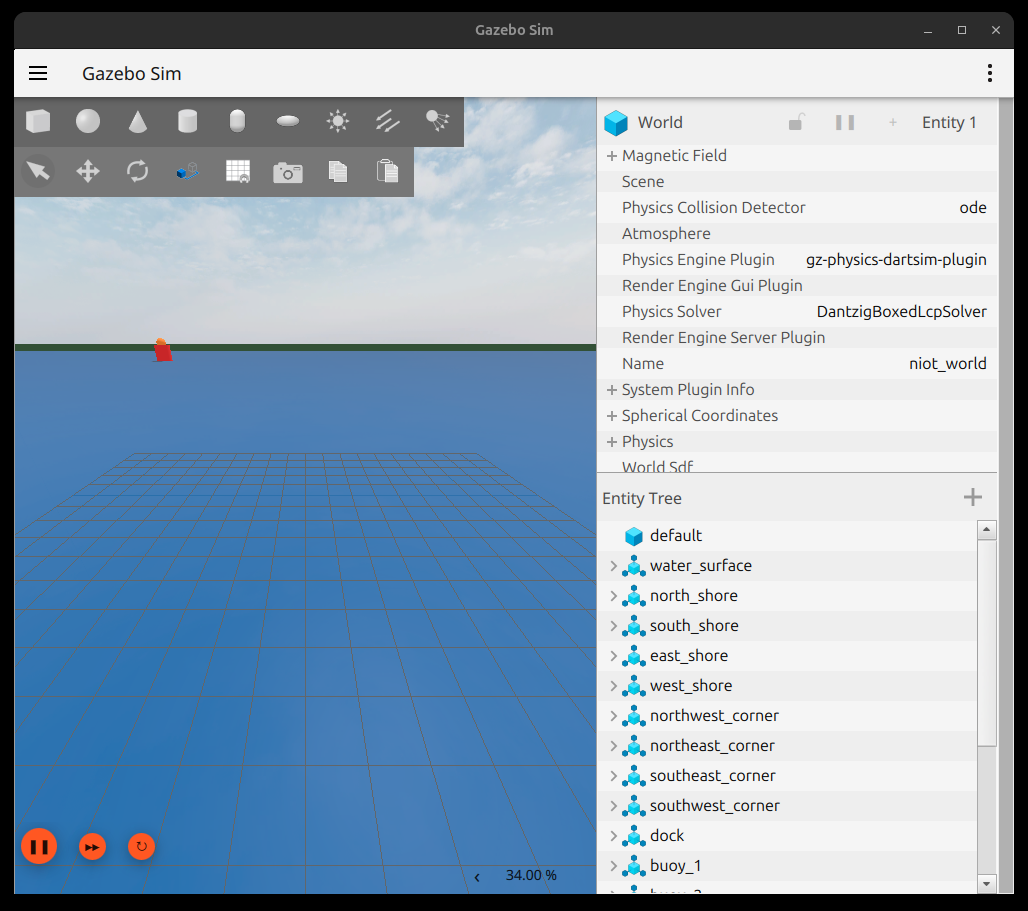
\includegraphics[width=0.88\textwidth]{figures/fig_gazebo_world.png}
  \caption{Gazebo Harmonic 3D simulation of the lake world and ASV plant
  (\texttt{niot\_world}).}
\end{figure}

\begin{figure}[H]
  \centering
  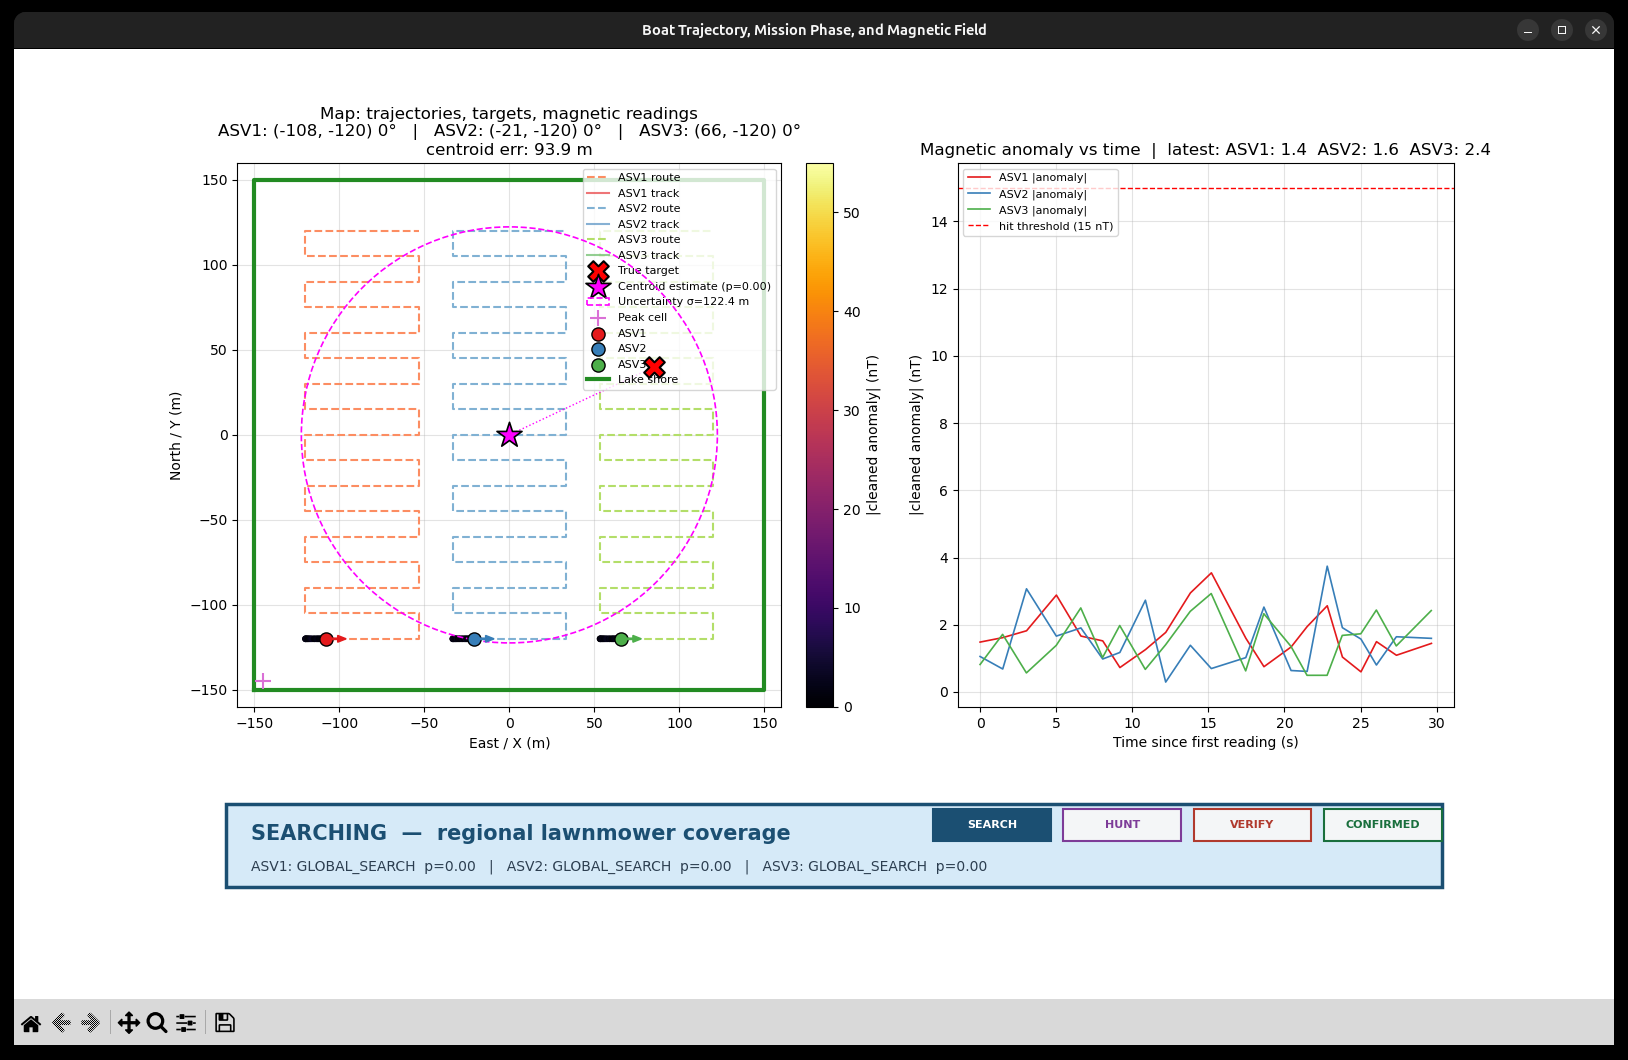
\includegraphics[width=0.92\textwidth]{figures/fig_operator_console_search.png}
  \caption{Operator console during SEARCH: three strip routes, true target
  marked, modes \texttt{GLOBAL\_SEARCH}.}
\end{figure}

\begin{figure}[H]
  \centering
  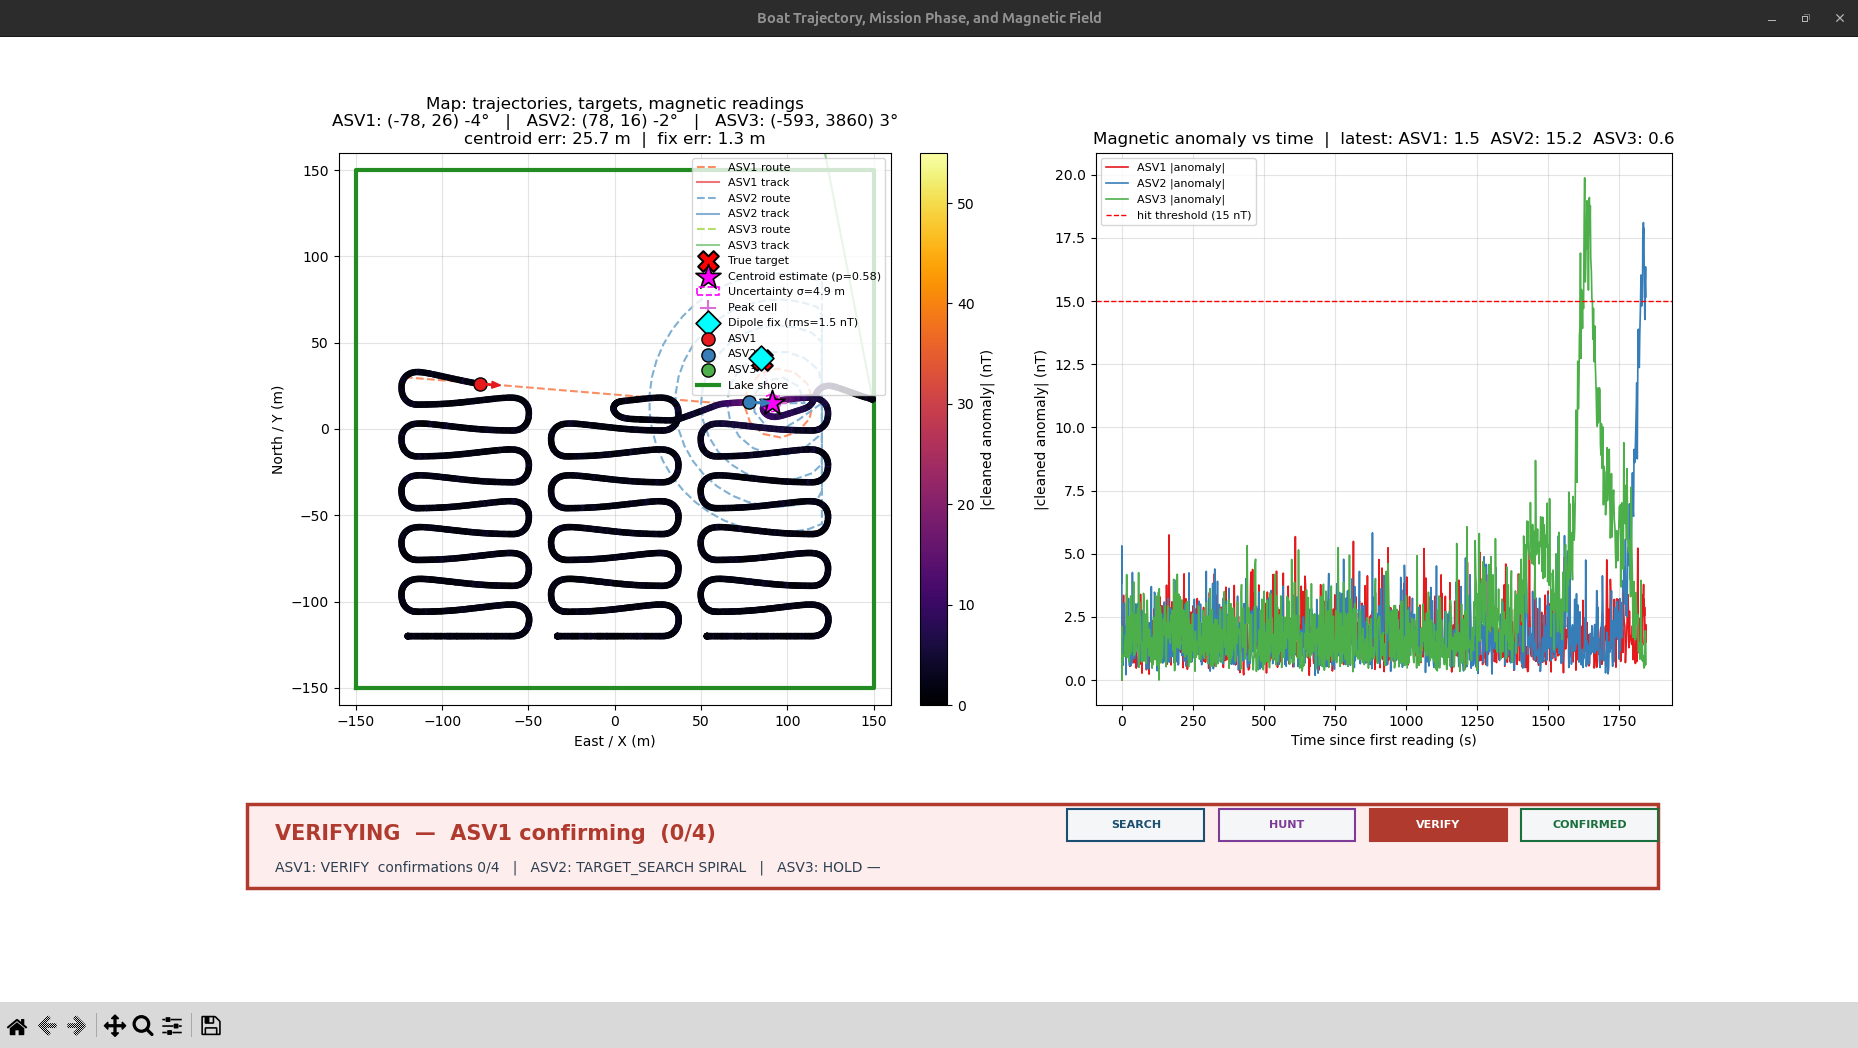
\includegraphics[width=0.92\textwidth]{figures/fig_hunt_verify_console.png}
  \caption{Hunt/VERIFY-era console: anomaly above $15\,\mathrm{nT}$ hit
  threshold and VERIFY phase indication.}
\end{figure}

\subsection{Obtained results and discussion}
A completed Phase-4 run produced:
\begin{center}
\begin{tabular}{@{}ll@{}}
\toprule
Mission outcome & \texttt{MISSION\_COMPLETE} \\
Verifier / confirmations & ASV1 / \textbf{4 of 4} \\
Declared candidate & $(95.0,15.0)$ by ASV3 ($p\!\approx\!0.956$) \\
Planted truth & $(85.0,40.0)$ \\
Best dipole-fix error $e_{\mathrm{fix}}$ & $\approx0.0\,\mathrm{m}$ (RMS $\approx1.4\,\mathrm{nT}$) \\
Median $e_{\mathrm{fix}}$ (last 50 fixes) & $\approx5.8\,\mathrm{m}$ \\
\bottomrule
\end{tabular}
\end{center}

\paragraph{Discussion.} Software COMPLETE validates the cooperative
discover--verify protocol. Early SEARCH centroid errors ($\sim90\,\mathrm{m}$)
are expected before HITs. During densified sampling, the continuum dipole fit
reaches metre-class agreement with the planted target, supporting the
theoretical chain from anomaly cleaning through Bayes fusion to LS refinement.
Shore-safe spiral sizing and non-verifier HOLD mitigate prior failure modes
(shore collider flings / dual spiral pile-up).

%-----------------------------------------------------------------------------
% 7. ACKNOWLEDGEMENTS
%-----------------------------------------------------------------------------
\section{Acknowledgements}
The authors thank \texttt{[INSTITUTE\_NAME]} for academic affiliation and
laboratory computing facilities supporting ROS~2 / Gazebo simulation; Faculty
Mentor \texttt{[FACULTY\_MENTOR\_NAME]} for guidance; and open-source
communities (ROS~2, Gazebo) for the middleware used in this PDR. Any funding
support will be listed here when applicable: \texttt{[FUNDING\_AGENCY\_IF\_ANY]}.

%-----------------------------------------------------------------------------
% 8. REFERENCES
%-----------------------------------------------------------------------------
\begin{thebibliography}{99}
\bibitem{ros2} Open Robotics, ``ROS~2 Jazzy documentation,''
\url{https://docs.ros.org/en/jazzy/}.
\bibitem{gz} Open Robotics, ``Gazebo Sim Harmonic,''
\url{https://gazebosim.org/}.
\bibitem{shannon} C.~E.~Shannon, ``A mathematical theory of communication,''
\emph{Bell Syst.\ Tech.\ J.}, vol.~27, pp.~379--423, 1948.
\bibitem{lm} K.~Levenberg, ``A method for the solution of certain non-linear
problems in least squares,'' \emph{Q.\ Appl.\ Math.}, vol.~2, pp.~164--168, 1944.
\bibitem{fossen} T.~I.~Fossen, \emph{Handbook of Marine Craft Hydrodynamics and
Motion Control}. Wiley, 2011.
\bibitem{uxo} Review literature on marine magnetic / UXO dipole surveys
(institutional library expansion recommended for camera-ready version).
\end{thebibliography}

\vspace{0.8cm}
\begin{center}
\footnotesize
Replace all \texttt{[PLACEHOLDERS]} before institutional submission.\\
Compile with pdfLaTeX; submit \textbf{PDF only} (target length 5--10 pages).
\end{center}

\end{document}
